\documentclass[12pt, a4paper]{article}
\usepackage{graphicx}

\newcommand{\url}[1]{\texttt{#1}}
\newcommand{\menu}[1]{\textbf{[#1]}}
\newcommand{\appName}{\texttt{SpiroJ}}
\renewcommand{\thepage}{\fbox{\arabic{page}}} 

\begin{document}

\section{Introduction}

\appName{} is a simple generator of hypotrochoids and similar roulettes. The basic principle is rolling one circle on another circle \cite{wikipedia}. SpiroJ tool is similar to the classic Spirograph toy, but it is more flexible. In addition, user can export generated roulettes to vector graphics, which can be imported to many graphic editors.

\section{Getting Started}

Run the \appName{} by clicking application JAR or using one of prepared batch files. You need Java\texttrademark{} Runtime Environment \cite{java} Version 1.4.x. or later to run the application (Version 1.4.2 is recommended).

Select \menu{File -- New Design} menu command. A default roulette should appear. Now you can try to change ratio value to 8 and press \menu{Calc} button, for example. Or try to decrease Rolling radius and calculate the roulette again. You can play with basic parameters and observe, how the shape changes.

\begin{figure}[ht]\centering
  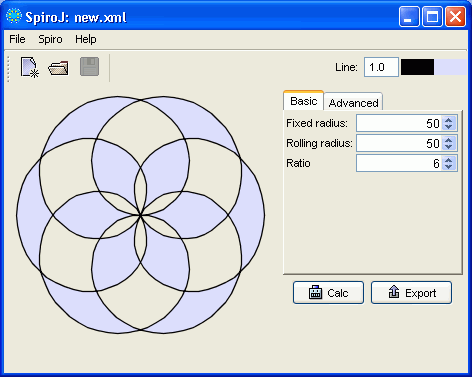
\includegraphics[width=10cm]{new_screen}
  \caption{New \appName{} design}
  \label{new_desing}
\end{figure}

Now, you can switch to the advanced tab and try more complex parameter adjustment. For your inspiration, you can load one of many example shapes from the \url{example} directory. If you want to understand details, please read mathematic description in section \ref{sec.mathem}.

\section{Exporting Image}

Current version of \appName{} can export to three vector formats:
\begin{itemize}
  \item Scalable Vector Graphics (SVG) -- based on XML and supported by W3C \cite{svg}. It becomes the internet standard for vector graphics.
  \item Encapsulated Postscript (EPS) -- standard vector graphics format, can be imported by Xara \cite{xara}.
  \item Adobe Illustrator 3.0 (AI) -- similar to EPS, also can be imported by Xara.
\end{itemize}

\section{Mathematics}\label{sec.mathem}

In the \appName{} application, the roulette is generated using cascade of two rotating operators (see Fig. \ref{doubleRot}). In basic mode (\ref{basic}), only radius $r$ of each rotation and frequency relation between them can be adjusted. In advanced mode (\ref{advanced}), radius and frequency for $x$ and $y$ axis can be adjusted separately for each rotation.

\begin{figure}[htp]\centering
  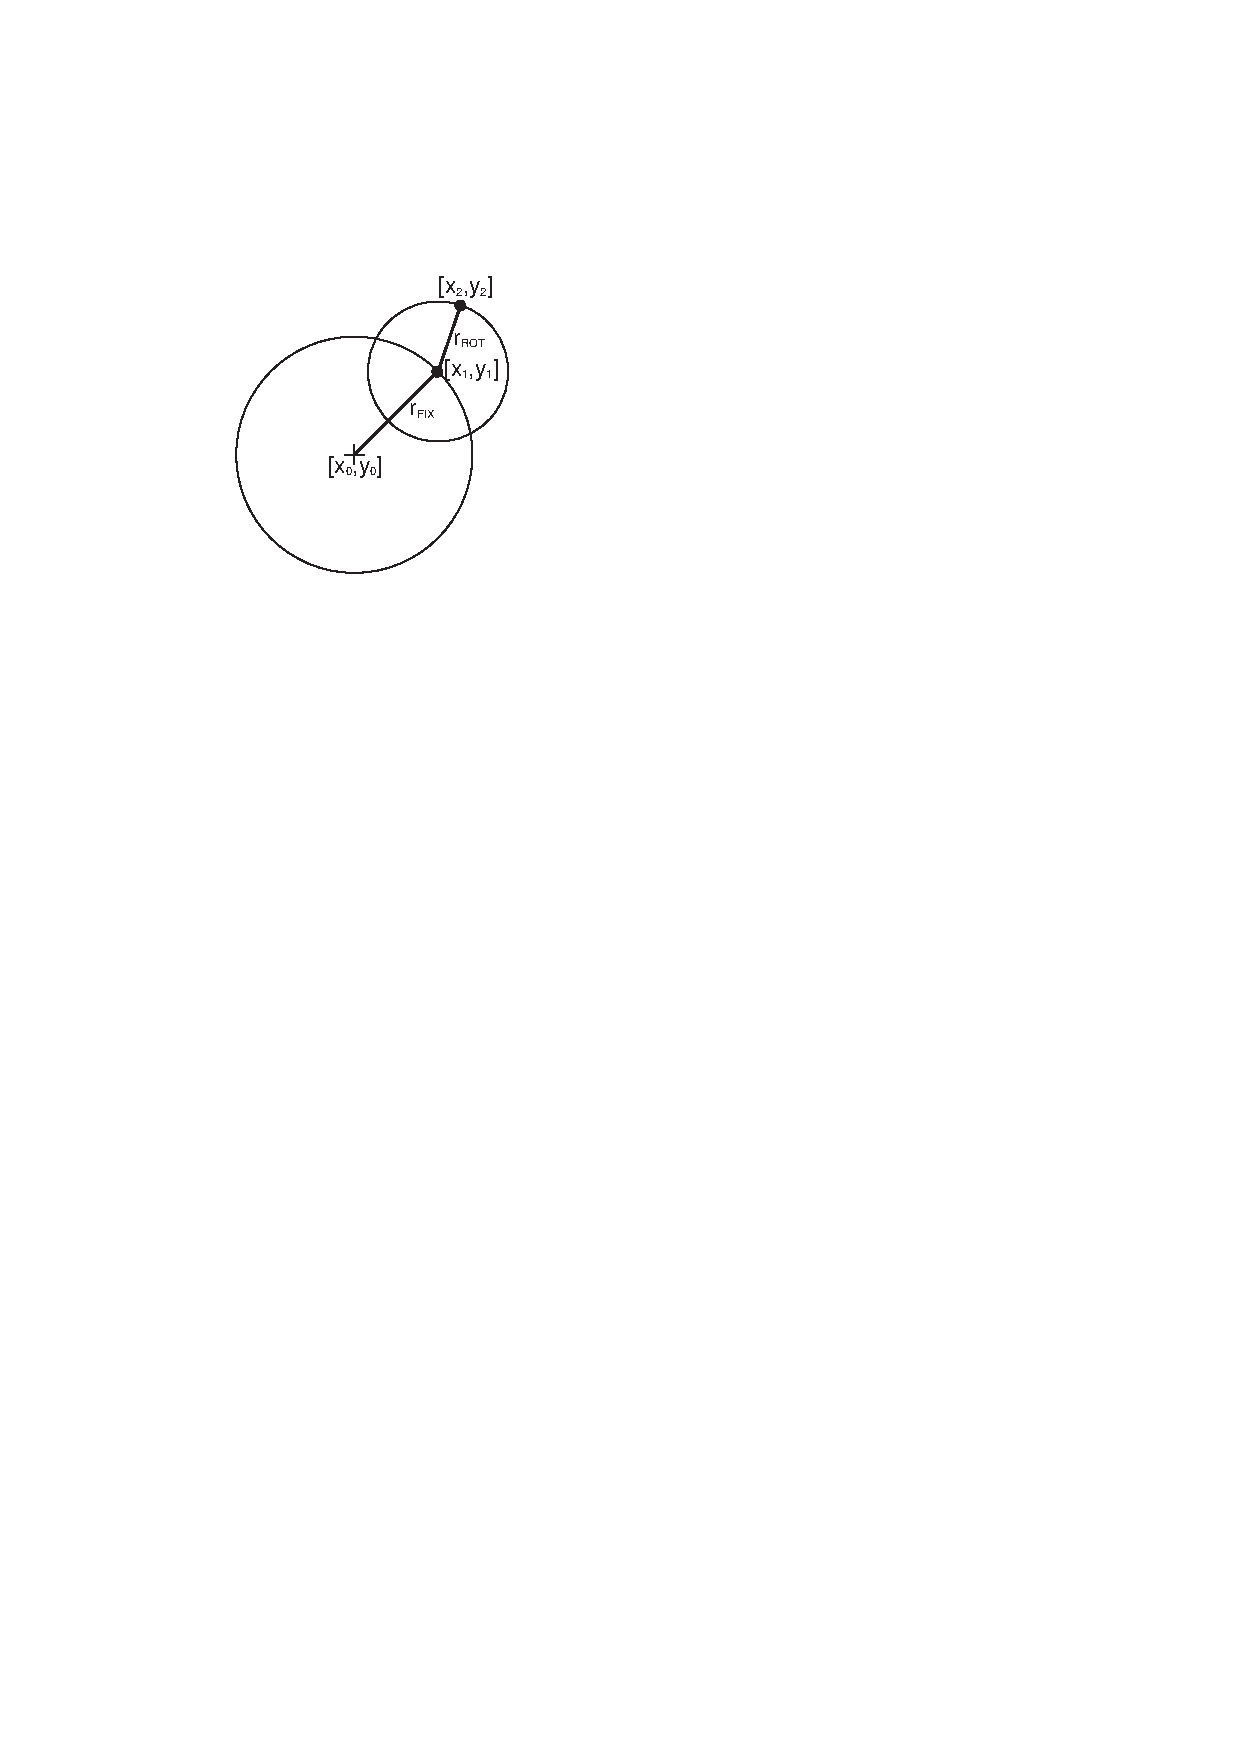
\includegraphics{math}
  \caption{Double rotation}
  \label{doubleRot}
\end{figure}

\begin{equation}\label{basic}
  \begin{array}{r@{\;=\;}l}
    x_{n+1} & x_n + r \cos{\alpha} \\
    y_{n+1} & y_n + r \sin{\alpha} 
  \end{array}
\end{equation}

\begin{equation}\label{advanced}
  \begin{array}{r@{\;=\;}l}
    x_{n+1} & x_n + r_x \cos(f_x s) \\
    y_{n+1} & y_n + r_y \sin(f_y s) 
  \end{array}
\end{equation}

The \appName{} user interface allows to edit only two rotating operators, but if you are familiar with XML, you can add more rotating operators to the chain by editing the XML and loading it into the application. In this case, you should understand what you are doing, of course.

\section{Examples}

You can emulate some classical curves. For example: switch to advanced mode and set $X$ radius to 60, $Y$ radius to 0 and both frequencies to 1 for fixed cycle, set $X$ radius to 0, $Y$ radius to 30 and both frequencies to 3 for rolling cycle, number of steps to 100, and you get a typical Lissajouse curve (\url{examples/lissajouse.xml}), see figure \ref{lissajouse}.

\begin{figure}[ht]\centering
  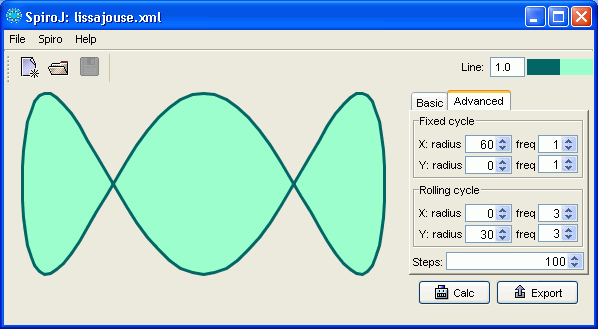
\includegraphics[width=10cm]{lissajouse_screen}
  \caption{Screen-shot: lissajouse.xml}
  \label{lissajouse}
\end{figure}

In the advanced mode, you can create very strange shapes. In the figure \ref{decor5sc} you can see screen-shot of the \appName{} and in the next figure is the same shape imported into Xara and slightly improved.

\begin{figure}[ht]\centering
  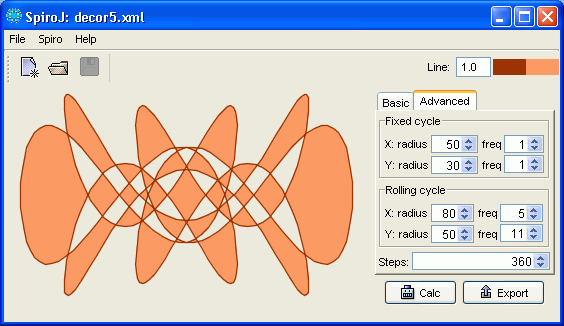
\includegraphics[width=10cm]{decor5_screen}
  \caption{Screen-shot: decor5.xml}
  \label{decor5sc}
\end{figure}

\begin{figure}[ht]\centering
  
\includegraphics[width=11cm]{decor5}
  \caption{Export from Xara Xtreme: decor5.pdf}
  \label{decor5}
\end{figure}

\begin{figure}[ht]\centering
  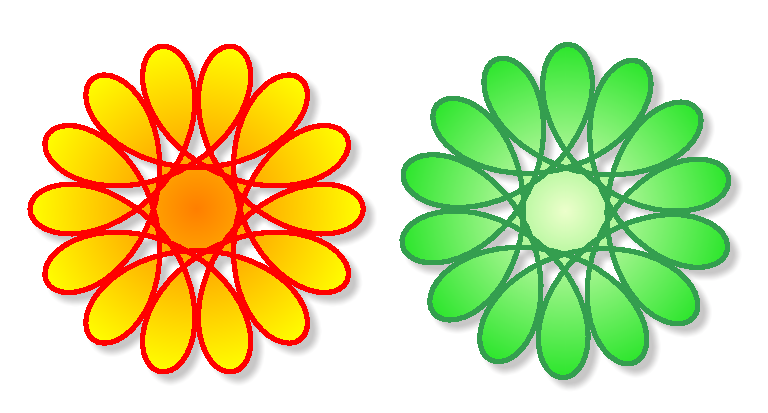
\includegraphics[width=11cm]{kvetina}
  \caption{Flower variations}
  \label{kvetina}
\end{figure}

\begin{figure}[ht]\centering
  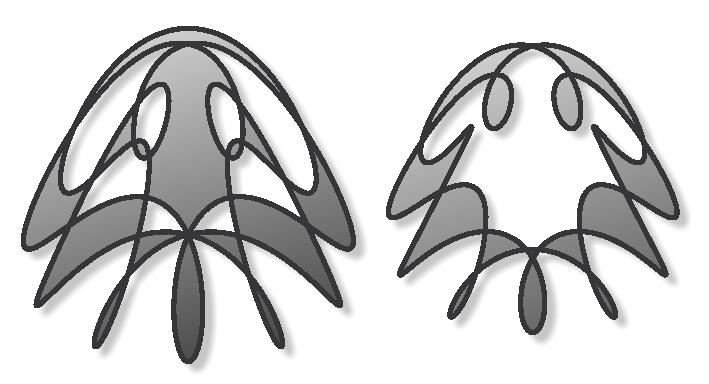
\includegraphics[width=11cm]{meduza}
  \caption{Jellyfish (medusa)}
  \label{meduza}
\end{figure}

\begin{figure}[ht]\centering
  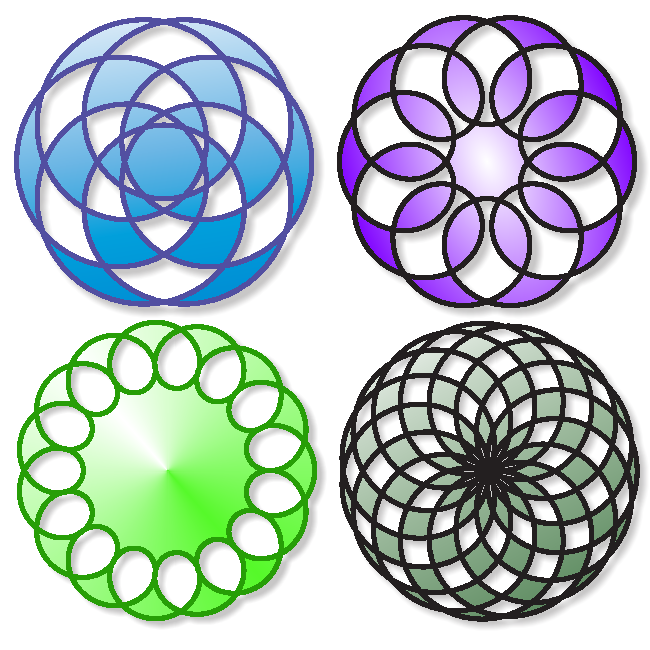
\includegraphics[width=11cm]{other}
  \caption{Other examples}
  \label{other}
\end{figure}


\clearpage
\begin{thebibliography}{99}
  \bibitem{wikipedia} \textsc{WikipediA}, The Free Encyclopedia, \url{http://www.wikipedia.org/} (Noveber 2005)
  \bibitem{java} Java Technology, \url{http://java.sun.com/} (November 2005)
  \bibitem{svg} Scalable Vector Graphics, \url{http://www.w3.org/Graphics/SVG/} (February 2006)
  \bibitem{xara} Web Graphics Software by Xara, \url{http://www.xara.com/} (February 2006)
\end{thebibliography} 

\end{document}
